% Chapter Template

\chapter{Implementation and Results} % Main chapter title

\label{Chapter2} % Change X to a consecutive number; for referencing this chapter elsewhere, use \ref{ChapterX}

%----------------------------------------------------------------------------------------
%	SECTION 1
%----------------------------------------------------------------------------------------

\section{Implementation}
The code base worked with, was a direct Fortran90 implementation of the fingerprint algorithm proposed by \cite{Zhu2016}. The compiler used for all computation was the GNU Fortran compiler \cite{gnufortran}.

\subsection{Data}
The data used were CNSTRUCTURES TODO with either 8 atoms per cell for \emph{training} and 16 atoms per cell for evaluation. The data was gathered by ... for ... . 

\begin{figure}[p]
\center
\label{fig:structures}
\subfloat[8 atom unit cell]{%
  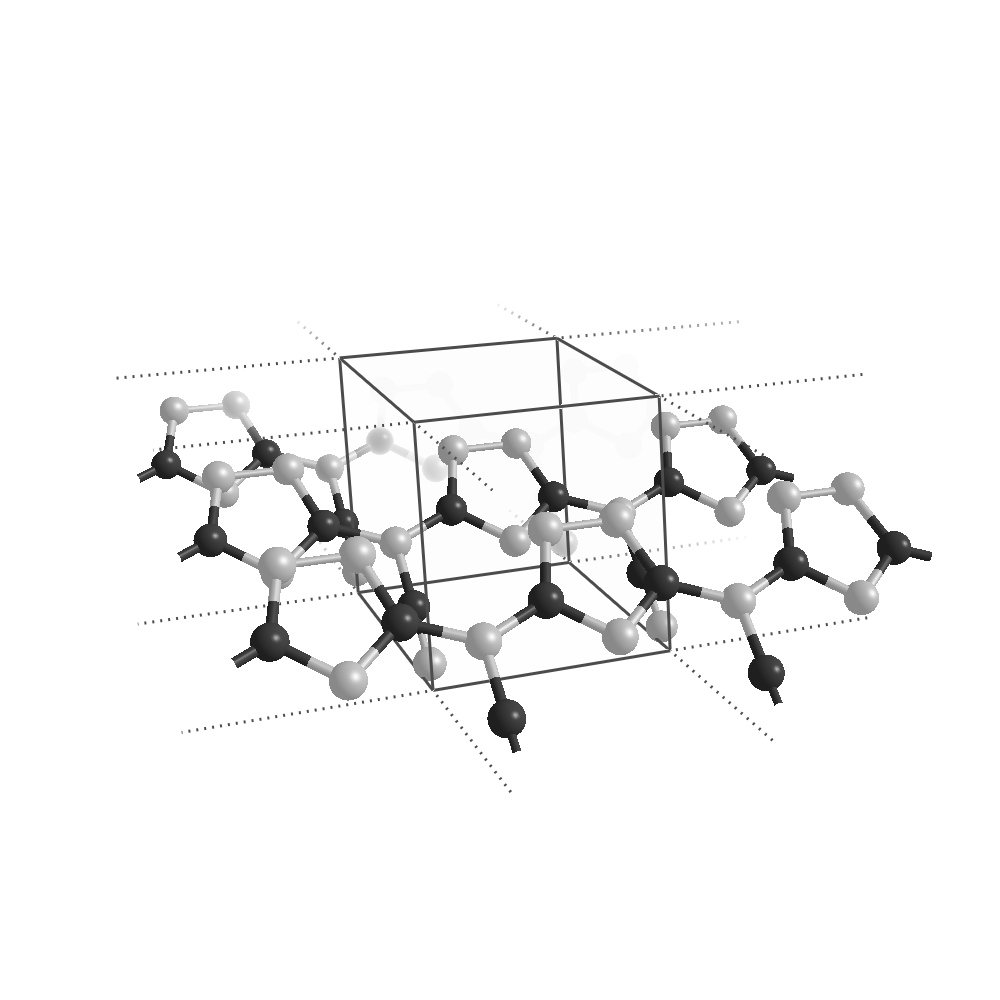
\includegraphics[clip,scale=0.3]{Figures/8structure.png}%
}

\subfloat[16 atom unit cell]{%
  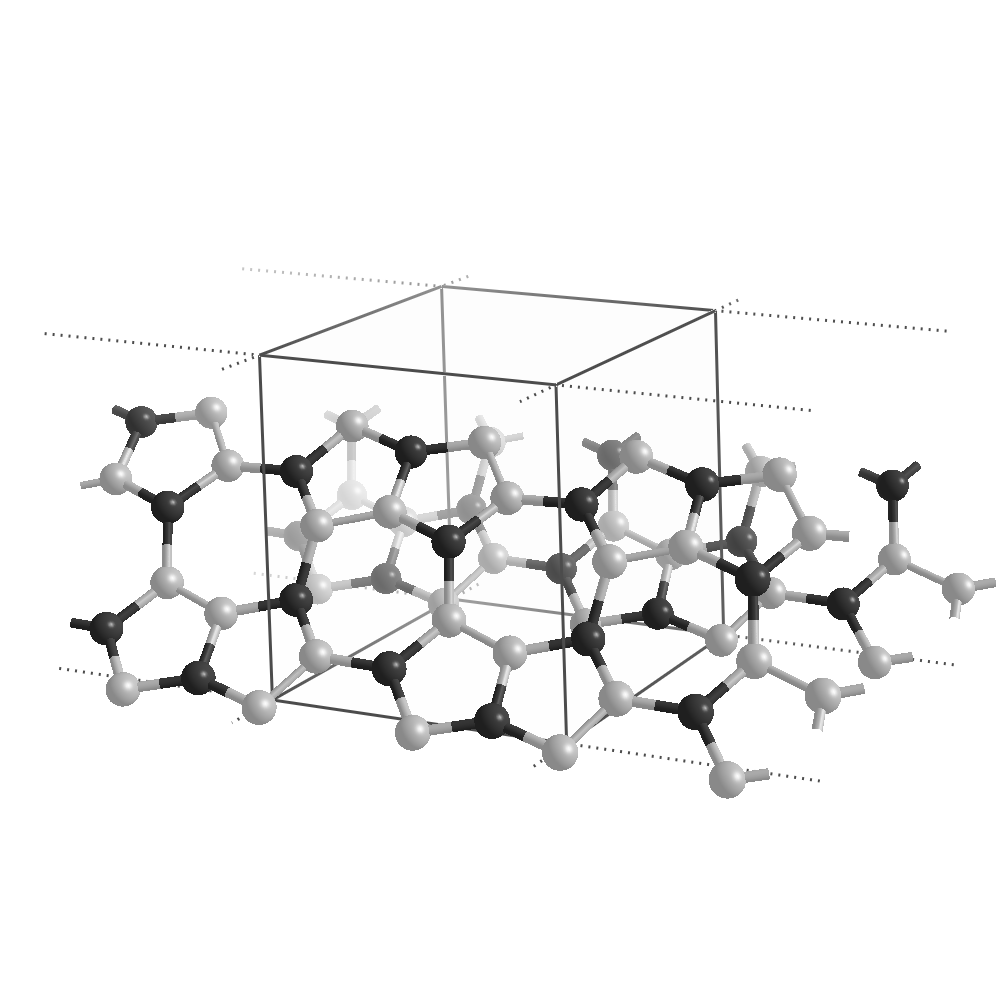
\includegraphics[clip,scale=0.3]{Figures/16structure.png}%
}

\caption{Example of the crystal structures used. C atoms are in black and N atoms in white. (A): Crystal sctructure with 8 atoms per cell. (B): Crystal structure with 16 atoms per cell.}

\end{figure}
\newpage
\subsection{Orbital Energies}
For calculating the overlap matrix (eq. \ref{ovrlap} ff.) the gaussian width $\alpha_i$ was originaly only dependent on the covalent radius of the respective atom type. This was further modified to respect the orbital eigenenergy of the respective orbital (eq. \ref{eq:const}). The values used were gathered from the NIST Atomic Reference Data for Electronic Stucture Calculations.

\begin{table}[h!]
\center
\label{table:energies}
\begin{tabular}{c|c|c}
            & \textbf{C} & \textbf{N} \\ \hline
2s {[}eV{]} & -0.500866  & -0.676151  \\ \hline
2p {[}eV{]} & -0.199186  & -0.266297 
\end{tabular}
\caption{2s and 2p orbital eigenenergies of N and C.}
\end{table}

The constant $C$ in (eq. \ref{eq:const}) was experimentally determined. To obtain a good resolution in comparing the fingerprints, the entries of the fingerprints should be reasonably large, but not to close to each other. One can see the effect of the constant $C$ out of (eq. \ref{eq:const}) by plotting the constant vs. the entries of the fingerprint.
With plots as seen in Figure \ref{fig:const} one can determine approximate boundaries for the constant. The entries should be reasonably distinct but still large enough to get a good resolution. The fine tuning was then done via maximizing the prediction accuracy. The final value used for all calculation was then $C=0.19$.


\begin{figure}[h]

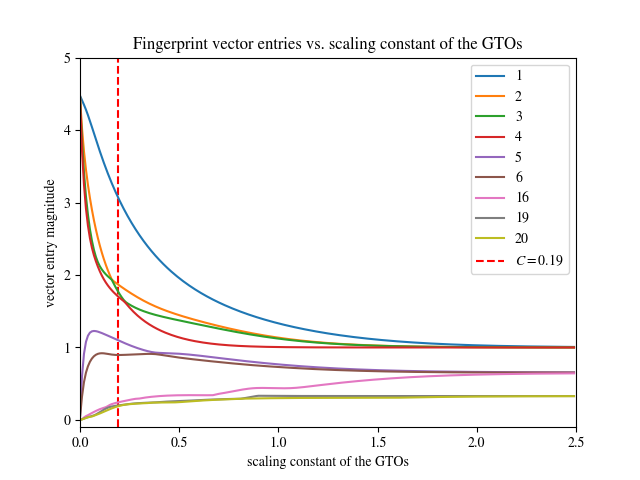
\includegraphics[width=\linewidth]{Figures/fpentry.png}
\caption{Plot of the fingerprint vector entries enumerated vs. the scaling constant of the GTO width.}
\label{fig:const} 
\end{figure}

\newpage
\section{Results}
\subsection{Landmark structures}

To calculate the landmark structures out of the fingerprints, we used a direct implementation of the algorithm maximum volume simplex method \cite{Behnam2020}. The task of this method should be to evaluate all atomar fingerprints given to it, and return the most distinct environments. These most distinct environments should furthermore each describe a different case of possible atomic environment regarding number of nearest neighbours (ligancy or coordination number) and type of nearest neighbours and their permutations. The method was evaluated on the set of 99 crystals with 8 atoms per crystal. Out of these 792 possible environments, the algorithm constructed a maximum volume simplex with 101 corners. A few of these landmark environments can be seen in Figure \ref{fig:landmarks}.
